\documentclass[twocolumn]{article}

\usepackage{graphicx}
\usepackage{fullpage}

\author{Juli\'{a}n Hern\'{a}ndez, Rodrigo Ipince, Jos\'{e} Mu\~{n}iz}
\title{A Comparison of Algorithms for Self Tuning Histograms}

\begin{document}

\maketitle


\begin{abstract}
In this paper, we explore the feasibility of implementing self-tuning histograms for OLTP databases. 
\end{abstract}


\section{Introduction}

Traditional database management systems based on the System-R design often include an optimizer. As explained in \cite{astrahan-76}, this optimizer is responsible for coming up with a low-cost query plan to execute. In order to estimate the costs of the set of feasible plans for a given query, the optimizer requires a selectivity. 

%What is a selectivity?

A common approach for estimating selectivities is to use a histogram associated with each field on each relation. The histogram captures the frequency of different values over a number of ranges.  Current commercial database systems like Oracle, Microsoft SQL Server, and Sybase, as well as open source alternatives like PostgreSQL and mySQL, all use this approach. 

Estimating the selectivity from a given query is easy and requires almost no overhead when consulting the histogram. However, the process of building a histogram is usually expensive. The previously mentioned database use a mechanism of statistical analysis by which they analyze the entire table after a threshold of insertions is met. This mechanism is, however, prohibitive when large-sized tables are constantly updated. This situation is common in OLTP transactions, and therefore is worth discussing.

% Introduce self tuning stuff

This paper is organized into seven parts. Section \ref{traditional-querying} describes how histograms are used in database systems. Section \ref{prev-work} shows some previous work on using results from queries to improve future cost estimates. Section \ref{our-work} then explains our modifications to the previous algorithms. Finally, Sections \ref{benchmark},  \ref{choice-queries}, and \ref{results} describe our framework for testing improvements for cost estimation over transactional loads. 





\section{Histogram querying and traditional building}\label{traditional-querying}
HI 

 As described in \cite{Gibbons-97}, a statistical approach to building histograms consists of 
 
 
\section{Previous self tuning histograms}\label{prev-work}

	\subsection{Curve fitting}
		\cite{Aboulnaga-99}

	\subsection{Aboulnaga }
 
\section{Modifications to proposed algorithms}\label{our-work}


\section{Benchmark setup}\label{benchmark}

% Why Postgres 

In order to test the accuracy of the previously discussed algorithms for self-tuning histograms, we built a system as shown in Figure \ref{pwngres-system} 

\begin{figure}
\begin{center}
	\label{pwngres-system}

	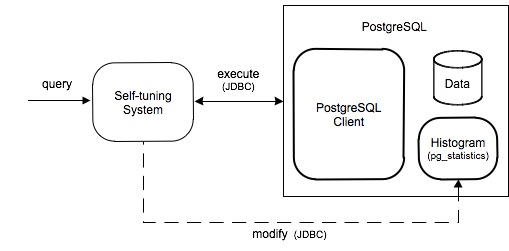
\includegraphics[width=0.8\columnwidth]{systemDiagram.JPEG}
	\caption{High level overview of the benchmarking system}	
\end{center}
\end{figure}

This system represents an intermediate layer between the end user and PostgreSQL, which intercepts the results from the database to the user and uses the cardinality to build a histogram. The different histograms can then be compared by their accuracy. 


This layer is responsible for receiving user queries. The information is then fetched back to Postgres, which responds to the middle system with the query plan to be executed. The benchmark tool then simulates the query plan, by reducing it into a family of nested loop joins and sequential scans with a set of conditions. For each query, a collection of \texttt{receive} calls is sent to the histogram builder. For each scan, the executor makes one \texttt{receive} �call. In the case of a join, for each element in the outer loop, the executor can make a \texttt{receive}  call as it matches the join field in the outer table with the tuples in the inner table. For example, if Tables \ref{emptable}� and \ref{depttable} are joined by a natural join, where \textbf{Employees} is the outer table, then we get the following three distinct \texttt{receive} calls: 

\begin{verbatim}
	 receive(``Dept.Country'', [3...3], 2)
	 receive(``Dept.Country'', [2...2], 0) 
	 receive(``Dept.Country'', [1...1], 1) 
\end{verbatim}
	
	\begin{table}
	\begin{center}
	\begin{tabular}[t]{|c|c|}
		\hline
		\textbf{EmpID} & \textbf{Country} \\
		\hline	
			1 		& 3			 \\
			2 		& 2			 \\
			3 		& 2			 \\
			4 		& 1			 \\
		\hline
	\end{tabular}
	\end{center}
	\label{emptable}
	\caption{Table for 	\textbf{Employees}�}
	\end{table}
	
	
	
	\begin{table}
	\begin{center}
	\begin{tabular}[t]{|c|c|}
		\hline
		\textbf{DeptID} & \textbf{Country} \\
		\hline	
			1 		& 3		          \\
			2 		& 3			 \\
			3 		& 1			 \\
		\hline
	\end{tabular}
	\end{center}
	\caption{Table for 	\textbf{Departments}�}
	\label{depttable}
	\end{table}
	
	






The system assumes independence between selectivities of multiple conditions, either over a single table or over several tables. In other words, if a query of the form \texttt{SELECT ... WHERE $p_1$ and $p_2$}, we assume that $\sigma_{p_1} \times \sigma_{p_2} = \sigma_{p_1 \land p_2}$.  For this reason, some joins operators might be able to send \texttt{receive}� messages even when facing multiple conditions, especially when one is a join condition and the other is a filter on the data. 


We chose not to modify the source code for Postgres directly for several reasons:

\begin{itemize}
	\item The s
	\item  
\end{itemize}

However, the benchmark still makes sense since all of Postgres implementation of joins, merge joins, hash joins and nested loops joins can all be modified to emit appropriately. 

Finally, it should be noted that we choose to measure our results in terms of row estimate errors, instead of query execution times. This decision was taken for several reasons :

\begin{itemize}	
	\item Modifying the \texttt{pg\_statistic} �table in Postgres,which is responsible for holding
		the histogram infromation, is not modifiable through an external interface. Although
		this histogram is stored in a table 
		
	\item Given that we do not consider the effect of join selectivity estimate errors from this paper, 
		we establish that a measurement of row selectivity in errors. 
	
	\item hej
	
	
\end{itemize}

\section{Choice of Queries and Insetions}\label{choice-queries}
We use a framework of insertions in the spirit of the TPC-C benchmark. We include the following tables:

\begin{enumerate}
	\item Customers
	\item Orders
	\item Products
\end{enumerate} 


\section{Results}\label{results}


\section{Conclusion}�



\section{Bibliography}

	\bibliographystyle{acm}
	\bibliography{Biblio}


\end{document}



%why this vs cq model. optimal for oltp txns with large loads, join selectivity still fails. 